\begin{figure}[!htbp]
    \center{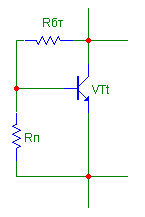
\includegraphics[width=0.24\linewidth]{picture_thermo_2}}
    \caption{Схема цепи термостабилизации}
    \label{figure:p2_2}
  \end{figure}

Цепь предназначена  для  создания  начального  смещения  на базах транзисторов выходного каскада. В процессе нагрева их параметры существенно изменяются, что влечет за собой изменение режимов и нарушение работы  всей  схемы. Цепь термостабилизации  в  зависимости  от  температурного  режима  изменяет  напряжение  смещения  так,  чтобы  компенсировать  изменение  параметров  транзисторов.\par Используем схему цепи термостабилизации, представленную на рисунке \ref{figure:p2_2}.\par
  Диапазон рабочих температур $-20\ldots +50~^0C$. \par